

% % % % % % % % % % % % % % % % % % % % % % % %


\documentclass[10pt,letterpaper]{article}
%\usepackage[top=0.85in,left=1.25in,footskip=0.75in]{geometry}


%fancy underlining from
%https://alexwlchan.net/2017/10/latex-underlines/

\usepackage{contour}
\usepackage{ulem}

\renewcommand{\ULdepth}{1.8pt}
\contourlength{0.8pt}

\newcommand{\myuline}[1]{%
  \uline{\phantom{\texttt{#1}}}%
  \llap{\contour{white}{\texttt{#1}}}%
}

\newcommand{\tts}{%
  \texttt{\,}
}

% amsmath and amssymb packages, useful for mathematical formulas and symbols
\usepackage{amsmath,amssymb}

% Use adjustwidth environment to exceed column width (see example table in text)
\usepackage{changepage}

% Use Unicode characters when possible
\usepackage[utf8x]{inputenc}

\usepackage{url}

% textcomp package and marvosym package for additional characters
\usepackage{textcomp,marvosym}

% cite package, to clean up citations in the main text. Do not remove.
\usepackage{cite}

% Use nameref to cite supporting information files (see Supporting Information section for more info)
%\usepackage{nameref,hyperref}

% line numbers
\usepackage{lineno}
\linenumbers

% ligatures disabled
\usepackage{microtype}
\DisableLigatures[f]{encoding = *, family = * }

% color can be used to apply background shading to table cells only
\usepackage[table]{xcolor}

% array package and thick rules for tables
\usepackage{array}

% create "+" rule type for thick vertical lines
\newcolumntype{+}{!{\vrule width 2pt}}

% create \thickcline for thick horizontal lines of variable length
\newlength\savedwidth
\newcommand\thickcline[1]{%
  \noalign{\global\savedwidth\arrayrulewidth\global\arrayrulewidth 2pt}%
  \cline{#1}%
  \noalign{\vskip\arrayrulewidth}%
  \noalign{\global\arrayrulewidth\savedwidth}%
}

% \thickhline command for thick horizontal lines that span the table
\newcommand\thickhline{\noalign{\global\savedwidth\arrayrulewidth\global\arrayrulewidth 2pt}%
\hline
\noalign{\global\arrayrulewidth\savedwidth}}

% Text layout
%\raggedright
%\setlength{\parindent}{0.5cm}
%\textwidth 5.25in 
%\textheight 8.75in

% Bold the 'Figure #' in the caption and separate it from the title/caption with a period
% Captions will be left justified
\usepackage[aboveskip=1pt,labelfont=bf,labelsep=period,justification=raggedright,singlelinecheck=off]{caption}
\renewcommand{\figurename}{Fig}


%tikz packages for drawing grammar trees
\usepackage{tikz}
\usepackage{tikz-qtree}
\usetikzlibrary{positioning}

% Use the PLoS provided BiBTeX style
%\bibliographystyle{plos2015}
%\usepackage{apacite}
%\bibliographystyle{apacite}
\bibliographystyle{abbrv}


%\usepackage[
%    backend=biber,
%    style=alphabetic,
%    citestyle=authoryear
%]{biblatex}

%some bibliography styles have a \citet mode which writes 
%Feckham et al (1953) instead of (Feckham et al, 1953) 
%plos2015 doesn't have this so this command replaces 
%\citet with \cite, 
%we can comment this out if we change to a 
%\citet supporting style.

\newcommand{\citet}[1]{\cite{#1}}

% Remove brackets from numbering in List of References
%\makeatletter
%\renewcommand{\@biblabel}[1]{\quad#1.}
%\makeatother

% Leave date blank
\date{}

%% Include all macros below

\newcommand{\lorem}{{\bf LOREM}}
\newcommand{\ipsum}{{\bf IPSUM}}

%% END MACROS SECTION


\begin{document}
\vspace*{0.2in}

% Title must be 250 characters or less.
\begin{flushleft}
{\Large
\textbf\newline{Grammatical category and the neural processing of phrases} 
}
\newline
% Insert author names, affiliations and corresponding author email (do not include titles, positions, or degrees).
\\
Amelia Burroughs\textsuperscript{1},
Nina Kazanina\textsuperscript{2,3},
Conor Houghton\textsuperscript{1*}
\\
\bigskip
\textsuperscript{1}Department of Computer Science, University of
Bristol, UK\\ \textsuperscript{2}School of Psychological Science,
University of Bristol, UK\\ \textsuperscript{3}International
Laboratory of Social Neurobiology, Institute for Cognitive
Neuroscience, National Research University Higher School of Economics,
Russian Federation \\
\bigskip

% Use the asterisk to denote corresponding authorship and provide email address in note below.
* conor.houghton@bristol.ac.uk

\end{flushleft}


\section*{Acknowledgements}
CJH and AB acknowledge support through a James S. McDonnell Foundation
Scholar Award in Cognition (JSMF \#220020239). NK acknowledges the
support of the HSE RF Government grant 075-15-2019-1930. We are
grateful to the anonymous referees for suggesting the behaviour
experiment and the `per-item' analysis.

% Please keep the abstract below 300 words
\section*{Abstract}

The interlocking roles of lexical, syntactic and semantic processing
in language comprehension has been the subject of longstanding
debate. Recently, the cortical response to a frequency-tagged
linguistic stimulus has been shown to track the rate of phrase and
sentence, as well as syllable, presentation. This could be interpreted
as evidence for the hierarchical processing of speech, or as a
response to the repetition of grammatical category. To examine the
extent to which hierarchical structure plays a role in language
processing we recorded EEG from human participants as they listen to
isochronous streams of monosyllabic words. Comparing responses to
sequences in which grammatical category is strictly alternating and
chosen such that two-word phrases can be grammatically constructed ---
\texttt{cold food loud room} --- or is absent --- \texttt{rough give
  ill tell} --- showed cortical entrainment at the two-word phrase
rate was only present in the grammatical condition. Thus, grammatical
category repetition alone does not yield entertainment at higher level
than a word. On the other hand, cortical entrainment was reduced for
the mixed-phrase condition that contained two-word phrases but no
grammatical category repetition --- \texttt{that word send less} ---
which is not what would be expected if the measured entrainment
reflected purely abstract hierarchical syntactic units. Our results
support a model in which word-level grammatical category information
is required to build larger units.

\section*{Introduction}

The ability of the human brain to rapidly generate meaning from an
incoming stream of words is an impressive feat. The role played by
hierarchical syntactic structure during this processing is the subject
of an ongoing debate with, on the two extremes, some arguing that full
hierarchical analysis is central to sentence comprehension
\citet{Chomsky1995,BerwickEtAl2013, EveraertEtAl2015}, while others
claim that hierarchical representations are non-essential
\cite{FrankEtAl2012, FrankBod2011, FrankYang2018,
  FrankChristiansen2018}.

According to the hierarchical account of language, comprehension is
underpinned by the brain's ability to abstract over a number of
linguistic levels, such as grammatical categories and phrases and to
combine them hierarchically according to a set of grammatical
principles. In this view language users parse an incoming sequence of
words into a nested tree-like structure that details taxonomy-like
relationships between syntactic constituents and enables sentence
comprehension (Fig.~\ref{fig:freq_tree}).

\begin{figure}[tb]
\begin{center}
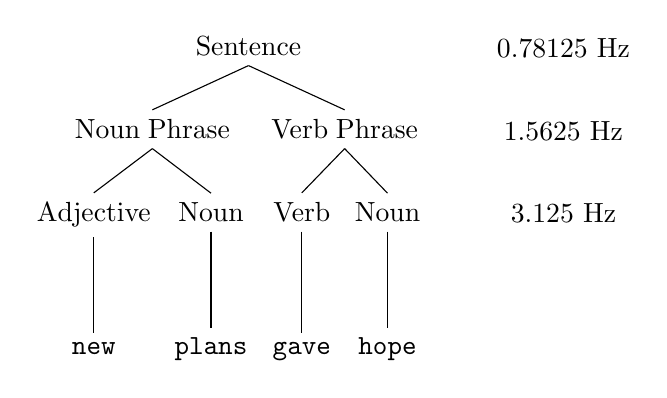
\begin{tikzpicture}
\tikzset{every tree node/.style={align=center,anchor=base}}
\tikzset{level 5+/.style={level distance=2\baselineskip}}
\tikzset{frontier/.style={distance from root=9\baselineskip}}
\Tree
    [.Sentence     
      [.Noun\;Phrase
        [.Adjective {\texttt{new}} ]
        [.Noun  {\texttt{plans}} ]
      ]
      [.Verb\;Phrase 
        [.Verb {\texttt{gave}} ]
        [.Noun {\texttt{hope}} ]
      ]
    ]
 \node at (4,0.1) {0.78125 Hz};
 \node at (4,-0.95) {1.5625 Hz};
 \node at (4,-2.0) {3.125 Hz};
\end{tikzpicture}
\end{center}
\caption{Demonstration of a syntactic tree for an example sentence
  from \cite{DingEtAl2016, DingEtAl2017}. The sentence is composed of
  a noun phrase and a verb phrase, each consisting of two words
  presented at a rate of 3.125 Hz.  The sentence is described using a
  hierarchical tree that splits the sentence first into a noun phrase
  and a verb phrase and then into words. This is a particularly simple
  tree, more complex trees may have more branches. This simple
  structure is convenient for frequency tagging and the different
  frequencies corresponding to the three levels of the tree, sentence,
  phrase and word, have been marked here.}
\label{fig:freq_tree}
\end{figure}

In support of this view, it has been demonstrated, using MEG in
\cite{DingEtAl2016} and using EEG in \cite{DingEtAl2017} that cortical
activity can entrain to the rate of syllable, phrase and sentence
presentation. In the EEG experiments participants were played
continuous streams of four-word sentences, where each word was 320 ms
long in duration and consisted of only a single syllable. As in
Fig.~\ref{fig:freq_tree} each sentence was composed of a noun phrase
and a verb phrase, each containing two words. Thus these stimuli
have a specific frequency at three levels of linguistic structure:
syllables at 3.125 Hz, phrases at 1.5625 Hz and sentences at 0.78125
Hz. The neural responses were analysed using time-frequency
decomposition and measures of inter-trial phase coherence
(ITPC). Cortical activity was found to be phase-locked to the rate of
presentation of syllables, phrases and sentences even though only the
syllable frequency was present in the auditory signal itself, the other
two frequencies rely on the meaning of the words and the structure of
the sentences.

However, it has also been suggested that the brain could rely on
simpler, potentially more generic, strategies underpinned by
statistical processing of linguistic representations. In line with
this, recent work \cite{FrankYang2018} has shown that a model solely
based on distributional word semantics is sufficient to predict the
response observed in \cite{DingEtAl2016, DingEtAl2017}. In this model
the distributional word semantics are represented by skipgram-word2vec
vectors \cite{MikolovEtAl2013,Bojanowski2017}. In skipgram, word2vec
vectors are calculated by training a simple linear neural network with
one hidden layer; the input and output layers both correspond to words
and the network is trained on the task of predicting, from a given
input word, the unordered list of words that occur in proximity to it
in text. The components of the word2vec vector for a given word are
the weights feeding forwards from the word to the hidden layer. Words
that are likely to occur in a similar context have similar
representations in the hidden layer and hence are associated with
similar word2vec vectors. To a striking degree these high-dimensional
vectors have specific directions that serve, at least locally, to
represent specific concepts, so that, for example, the same direction
that leads from ``big'' to ``biggest'' leads from ``small'' to
``smallest'' \cite{MikolovEtAl2013b, MikolovEtAl2013c}.

In \citet{FrankYang2018} fictive EEG signals representing experimental
trials were constructed from the word2vec vectors for each
stimulus. In the EEG experiment each word was presented for 320 ms and
so, in the ficitive data 320 copies of the vector for each word were
lined up side-by-side forming the columns of a matrix so each column
represents 1 ms of the stimulus. The rows of this matrix were then
treated as a EEG and this fictive signal was analysed in the same way
as the real EEG signal is, with measures of the evoked response
averaged over rows, much as we average over individual
electrodes. This simulated EEG signal demonstrated the same
entrainment to words, phrases and sentences as the real signal. Since
the high-dimensional word2vec vectors represent single words only and
do not explicitly encode information about word sequences, this
demonstrated that semantic relationships that can be deduced from a
text corpus are sufficient to explain the ITPC peaks seen in the real
experiment, without any need to invoke the hierarchical structure of
the sentence.

The current study aimed to elucidate the importance of hierarchical
structure during language processing using EEG. We recorded neural
activity from 20 participants while they listened to streams of
two-word sequences from four different conditions:
\begin{enumerate}
    \item[AN] (adjective-noun): repetition of adjective-noun sequences, 
    \item[AV] (adjective-verb): repetition of adjective-verb sequences, 
    \item[MP] (mixed phrase): repetition of grammatical two-word phrases with varying grammatical categories, 
    \item [RR] (random): random word order; no phrases possible.
\end{enumerate}
In the AN and AV conditions, grammatical categories occurred at a regular
rate, so adjectives, nouns or verbs were repeated every other
word. However the stream could only be parsed into grammatical phrases
in the AN condition, for example:
\begin{center}
  \begin{tabular}{cl}
   &\texttt{A}\tts\tts{}\tts{}\tts{}\texttt{N}\tts\tts{}\tts{}\tts{}\texttt{A}\tts\tts{}\tts{}\tts{}\texttt{N}\tts\tts{}\tts{}\tts{}\texttt{A}\tts\tts{}\tts{}\tts{}\texttt{N}\\ 
AN:&\myuline{cold food}\tts\myuline{loud room}{}\tts\myuline{tall girl}
\end{tabular}
  \end{center}
where underlining indicates grammatical phrases. In the AV condition, no such grammatical phrases
could be formed, as in the example:
\begin{center}
  \begin{tabular}{cl}
   &\texttt{A}\tts\tts{}\tts{}\tts{}\tts{}\texttt{V}\tts\tts{}\tts{}\tts{}\texttt{A}\tts{}\tts{}\tts{}\texttt{V}\tts\tts{}\tts{}\tts{}\texttt{A}\tts\tts{}\tts{}\tts{}\texttt{V}\\ 
AV:&\texttt{rough give}\tts\texttt{ill tell}{}\tts\texttt{thin chew}
\end{tabular}
  \end{center}
In the MP condition, grammatical two-word phrases could be formed, but
grammatical category occurred with no regularity, for example
\begin{center}
  \begin{tabular}{cl}
   &\texttt{Det}\tts{}\tts{}\texttt{N}\tts\tts{}\tts{}\tts{}\texttt{V}\tts{}\tts\tts{}\tts{}\texttt{P}\tts\tts{}\tts{}\tts{}\texttt{Adv}\tts{}\texttt{V}\\ 
MP:&\myuline{that word}\tts\myuline{send less}{}\tts\myuline{too loud}
\end{tabular}
\end{center}
and, finally, in the RR condition there are neither grammatical phrases nor any regularity
\begin{center}
  \begin{tabular}{cl}
   &\texttt{Pre}\tts{}\tts{}\texttt{V}\tts\tts\tts{}\tts{}\tts{}\texttt{A}\tts{}\tts\tts{}\tts{}\texttt{P}\tts{}\tts{}\tts{}\texttt{V}\tts\tts\tts\tts{}\texttt{Det}\\ 
RR:&\texttt{from solve}\tts\texttt{good him}{}\tts\texttt{ask an}
\end{tabular}
\end{center}

As in \cite{DingEtAl2017} the principle measure of response used here
is the inter-trial phase coherence (ITPC); this quantifies the
clustering of phases across trials at a given frequency. According to
the hierarchical account we would expect a peak in ITPC at the phrase
rate in both the AN and MP conditions, but no peak in ITPC in the AV
or RR condition. A sequential account of language processing that
relies primarily upon word-level statistics would instead predict a
peak in ITPC at the phrasal rate in both the AN and AV conditions: our
stimulus was designed so that the peak calculated using the
fictive EEG simulated from word2vec gives similar phrase peaks in the
AN and AV conditions.

Anticipating the main results, a peak in ITPC at the phrasal rate was
significantly larger for AN than for any of the other conditions,
suggesting that neural entrainment cannot be explained solely by
hierarchical accounts or grammatical category regularity; rather, it
additionally calls for higher level, syntactic representations. Our
results support a language system that exploits both linear and
hierarchical operations of language inputs to generate meaning.

\section*{Results}

\begin{figure}[tbhp]
%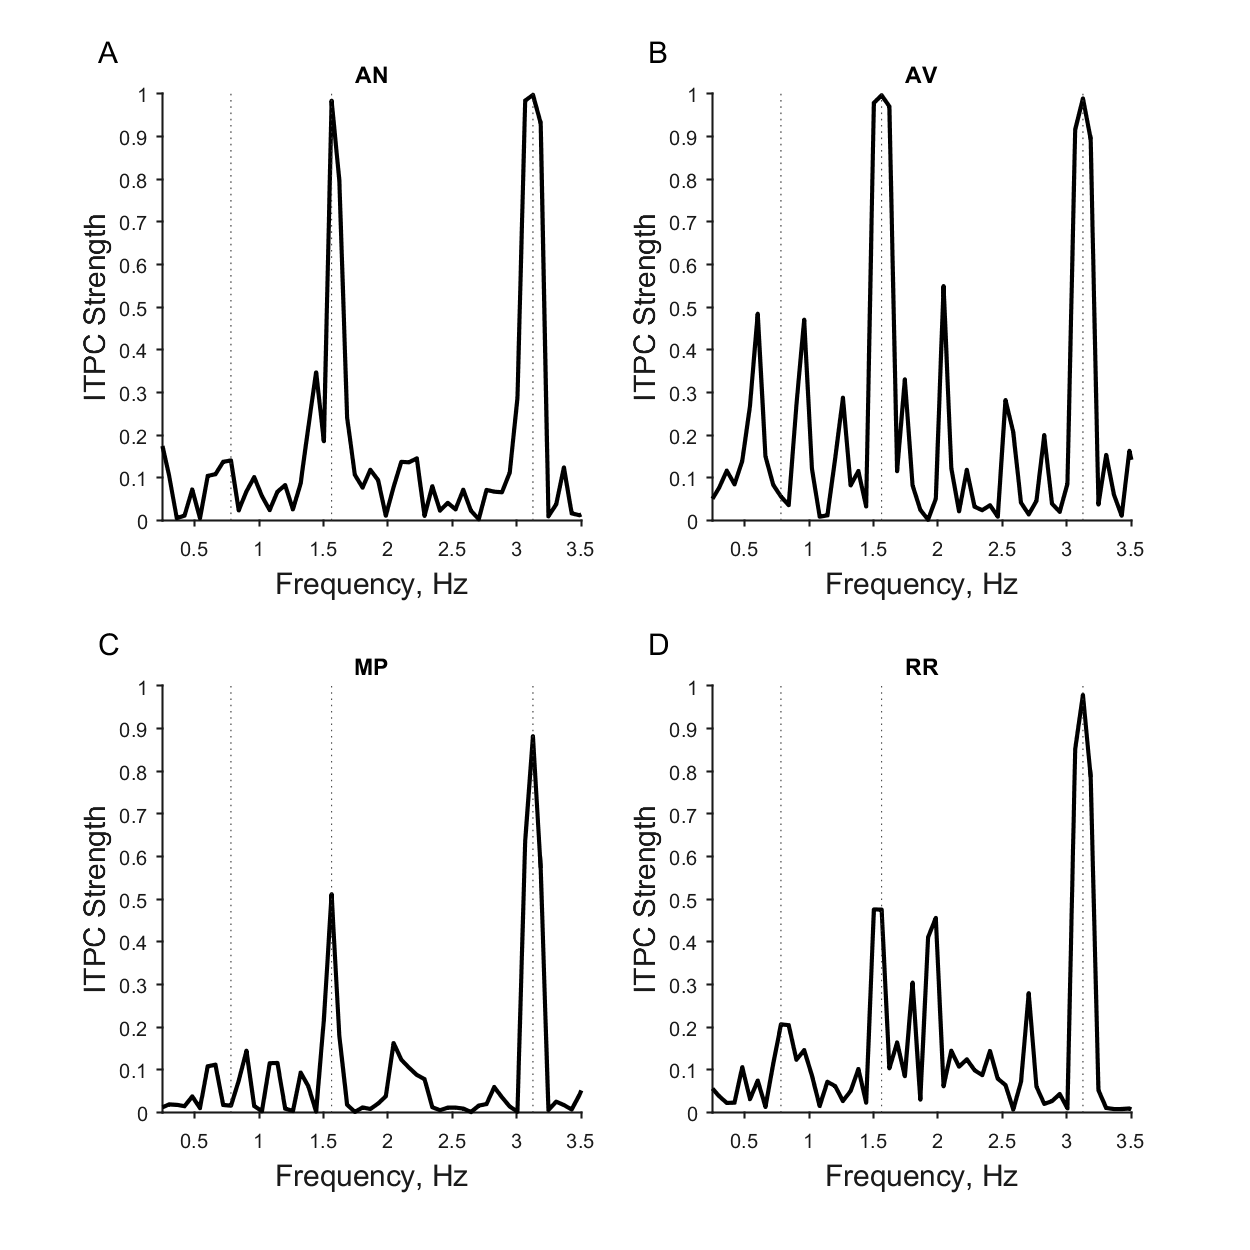
\includegraphics[width=\linewidth]{FrankFigure_exp2_phrases_12_03_2020.png}
% GNUPLOT: LaTeX picture with Postscript
\begingroup
  \makeatletter
  \providecommand\color[2][]{%
    \GenericError{(gnuplot) \space\space\space\@spaces}{%
      Package color not loaded in conjunction with
      terminal option `colourtext'%
    }{See the gnuplot documentation for explanation.%
    }{Either use 'blacktext' in gnuplot or load the package
      color.sty in LaTeX.}%
    \renewcommand\color[2][]{}%
  }%
  \providecommand\includegraphics[2][]{%
    \GenericError{(gnuplot) \space\space\space\@spaces}{%
      Package graphicx or graphics not loaded%
    }{See the gnuplot documentation for explanation.%
    }{The gnuplot epslatex terminal needs graphicx.sty or graphics.sty.}%
    \renewcommand\includegraphics[2][]{}%
  }%
  \providecommand\rotatebox[2]{#2}%
  \@ifundefined{ifGPcolor}{%
    \newif\ifGPcolor
    \GPcolorfalse
  }{}%
  \@ifundefined{ifGPblacktext}{%
    \newif\ifGPblacktext
    \GPblacktexttrue
  }{}%
  % define a \g@addto@macro without @ in the name:
  \let\gplgaddtomacro\g@addto@macro
  % define empty templates for all commands taking text:
  \gdef\gplbacktext{}%
  \gdef\gplfronttext{}%
  \makeatother
  \ifGPblacktext
    % no textcolor at all
    \def\colorrgb#1{}%
    \def\colorgray#1{}%
  \else
    % gray or color?
    \ifGPcolor
      \def\colorrgb#1{\color[rgb]{#1}}%
      \def\colorgray#1{\color[gray]{#1}}%
      \expandafter\def\csname LTw\endcsname{\color{white}}%
      \expandafter\def\csname LTb\endcsname{\color{black}}%
      \expandafter\def\csname LTa\endcsname{\color{black}}%
      \expandafter\def\csname LT0\endcsname{\color[rgb]{1,0,0}}%
      \expandafter\def\csname LT1\endcsname{\color[rgb]{0,1,0}}%
      \expandafter\def\csname LT2\endcsname{\color[rgb]{0,0,1}}%
      \expandafter\def\csname LT3\endcsname{\color[rgb]{1,0,1}}%
      \expandafter\def\csname LT4\endcsname{\color[rgb]{0,1,1}}%
      \expandafter\def\csname LT5\endcsname{\color[rgb]{1,1,0}}%
      \expandafter\def\csname LT6\endcsname{\color[rgb]{0,0,0}}%
      \expandafter\def\csname LT7\endcsname{\color[rgb]{1,0.3,0}}%
      \expandafter\def\csname LT8\endcsname{\color[rgb]{0.5,0.5,0.5}}%
    \else
      % gray
      \def\colorrgb#1{\color{black}}%
      \def\colorgray#1{\color[gray]{#1}}%
      \expandafter\def\csname LTw\endcsname{\color{white}}%
      \expandafter\def\csname LTb\endcsname{\color{black}}%
      \expandafter\def\csname LTa\endcsname{\color{black}}%
      \expandafter\def\csname LT0\endcsname{\color{black}}%
      \expandafter\def\csname LT1\endcsname{\color{black}}%
      \expandafter\def\csname LT2\endcsname{\color{black}}%
      \expandafter\def\csname LT3\endcsname{\color{black}}%
      \expandafter\def\csname LT4\endcsname{\color{black}}%
      \expandafter\def\csname LT5\endcsname{\color{black}}%
      \expandafter\def\csname LT6\endcsname{\color{black}}%
      \expandafter\def\csname LT7\endcsname{\color{black}}%
      \expandafter\def\csname LT8\endcsname{\color{black}}%
    \fi
  \fi
  \setlength{\unitlength}{0.0500bp}%
  \begin{picture}(6000.00,4500.00)%
    \gplgaddtomacro\gplbacktext{%
      \csname LTb\endcsname%
      \put(946,704){\makebox(0,0)[r]{\strut{} 0}}%
      \put(946,1014){\makebox(0,0)[r]{\strut{} 0.2}}%
      \put(946,1325){\makebox(0,0)[r]{\strut{} 0.4}}%
      \put(946,1635){\makebox(0,0)[r]{\strut{} 0.6}}%
      \put(946,1946){\makebox(0,0)[r]{\strut{} 0.8}}%
      \put(946,2256){\makebox(0,0)[r]{\strut{} 1}}%
      \put(1078,484){\makebox(0,0){\strut{} 0}}%      
      \put(1609,484){\makebox(0,0){\strut{} 1}}%      
      \put(2141,484){\makebox(0,0){\strut{} 2}}%      
      \put(2672,484){\makebox(0,0){\strut{} 3}}%      
      \put(3203,484){\makebox(0,0){\strut{} 4}}%
      \put(376,1480){\rotatebox{-270}{\makebox(0,0){\strut{}ITPC}}}%
      \put(2140,154){\makebox(0,0){\strut{}frequency, Hz}}%
      \put(2141,2400){\makebox(0,0){\strut{} \bf{MP}}}%             


      \put(3946,704){\makebox(0,0)[r]{\strut{} 0}}%
      \put(3946,1014){\makebox(0,0)[r]{\strut{} 0.2}}%
      \put(3946,1325){\makebox(0,0)[r]{\strut{} 0.4}}%
      \put(3946,1635){\makebox(0,0)[r]{\strut{} 0.6}}%
      \put(3946,1946){\makebox(0,0)[r]{\strut{} 0.8}}%
      \put(3946,2256){\makebox(0,0)[r]{\strut{} 1}}%
      \put(4078,484){\makebox(0,0){\strut{} 0}}%      
      \put(4609,484){\makebox(0,0){\strut{} 1}}%      
      \put(5141,484){\makebox(0,0){\strut{} 2}}%      
      \put(5672,484){\makebox(0,0){\strut{} 3}}%      
      \put(6203,484){\makebox(0,0){\strut{} 4}}%
%      \put(3176,1480){\rotatebox{-270}{\makebox(0,0){\strut{}ITPC}}}%
      \put(5140,154){\makebox(0,0){\strut{}frequency, Hz}}%
      \put(5141,2400){\makebox(0,0){\strut{} \bf{random}}}%             

      \put(946,3004){\makebox(0,0)[r]{\strut{} 0}}%
      \put(946,3314){\makebox(0,0)[r]{\strut{} 0.2}}%
      \put(946,3625){\makebox(0,0)[r]{\strut{} 0.4}}%
      \put(946,3935){\makebox(0,0)[r]{\strut{} 0.6}}%
      \put(946,4246){\makebox(0,0)[r]{\strut{} 0.8}}%
      \put(946,4556){\makebox(0,0)[r]{\strut{} 1}}%
      \put(1078,2784){\makebox(0,0){\strut{} 0}}%
      \put(1609,2784){\makebox(0,0){\strut{} 1}}%      
      \put(2141,2784){\makebox(0,0){\strut{} 2}}%      
      \put(2672,2784){\makebox(0,0){\strut{} 3}}%      
      \put(3203,2784){\makebox(0,0){\strut{} 4}}%
      \put(376,3980){\rotatebox{-270}{\makebox(0,0){\strut{}ITPC}}}%
            \put(2141,4700){\makebox(0,0){\strut{} \bf{AN}}}%      
 %     \put(2140,2154){\makebox(0,0){\strut{}frequency, Hz}}%

      \put(3946,3004){\makebox(0,0)[r]{\strut{} 0}}%
      \put(3946,3314){\makebox(0,0)[r]{\strut{} 0.2}}%
      \put(3946,3625){\makebox(0,0)[r]{\strut{} 0.4}}%
      \put(3946,3935){\makebox(0,0)[r]{\strut{} 0.6}}%
      \put(3946,4246){\makebox(0,0)[r]{\strut{} 0.8}}%
      \put(3946,4556){\makebox(0,0)[r]{\strut{} 1}}%
      \put(4078,2784){\makebox(0,0){\strut{} 0}}%      
      \put(4609,2784){\makebox(0,0){\strut{} 1}}%      
      \put(5141,2784){\makebox(0,0){\strut{} 2}}%      
      \put(5672,2784){\makebox(0,0){\strut{} 3}}%      
      \put(6203,2784){\makebox(0,0){\strut{} 4}}%
                  \put(5141,4700){\makebox(0,0){\strut{} \bf{AV}}}%             
 %     \put(3176,4480){\rotatebox{-270}{\makebox(0,0){\strut{}ITPC}}}%
 %     \put(5140,2154){\makebox(0,0){\strut{}frequency, Hz}}%
}%
    \gplgaddtomacro\gplfronttext{%
    }%
    \gplbacktext
    \put(0,2300){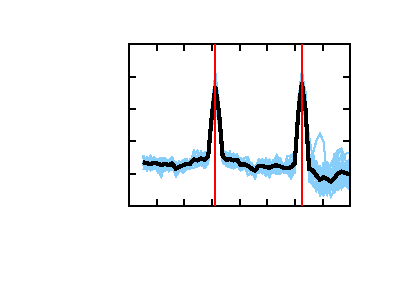
\includegraphics{./Figure_Simulated/anan_simulated}}%TL
    \put(3000,2300){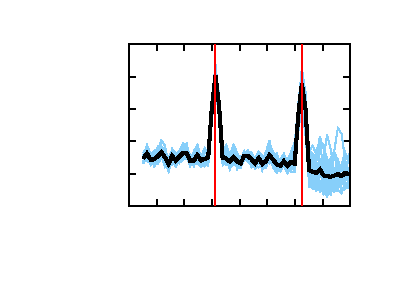
\includegraphics{./Figure_Simulated/avav_simulated}}%TR    
    \put(0,0){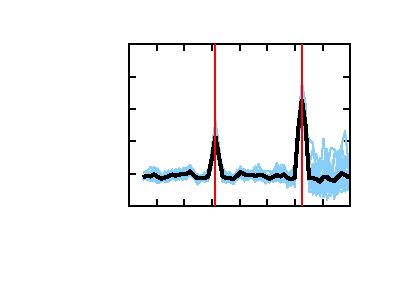
\includegraphics{./Figure_Simulated/phmi_simulated}}%BL
    \put(3000,0){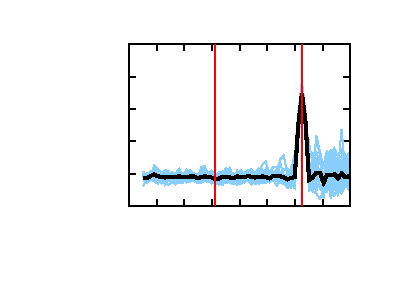
\includegraphics{./Figure_Simulated/rrrr_simulated}}%BR
    \gplfronttext
  \end{picture}%
\endgroup

\caption{ITPC of the simulated EEG calculated from the word2vec
  representation for the four conditions. The model yielded peaks in
  ITPC at the rate of syllable presentation (3.125 Hz) in each of the
  four conditions (AN, AV, MP, random). Vertical red lines represent
  the frequency at which syllables and two-word sequences are
  presented, the blue lines show responses for 20 simulated
  particants, the black is the grand average over these participants.
}
\label{fig:Fig1}
\end{figure}

The simulated EEG calculated from the word2vec representation yielded
a peak in ITPC of the simulated EEG responses at the rate of syllable
presentation (3.125 Hz, Fig.~\ref{fig:Fig1} in each of the four
conditions. The model also yielded a peak in ITPC at the rate of
phrase presentation (1.5625 Hz) for the AN and AV conditions
(~\ref{fig:Fig1}), where, respectively, the grammatical adjective-noun
phrases or the ungrammatical adjective-verb sequences were repeatedly
presented. As described in the Methods, the stimuli for the AN and AV
conditions were designed so that the vectors corresponding to
successive words have similar distances in both of these conditions
and the AN and AV conditions show similar peaks at the phrase
frequency, even though one condition can be parsed into grammatical
two-word phrases and the other cannot. The model also showed a
pronounced, but lower amplitude peak in ITPC at the rate of phrase
presentation during the MP condition. The phrase peak was absent from
an version of the RR condition in which words are shuffled at random.

Human EEG data showed a highly significant peak ($p<10^{-6}$) in ITPC
at the rate of syllable presentation (3.125 Hz) in all conditions
tested (Fig.~\ref{fig:Fig2}). There was a highly prominent peak at the
phrase rate (1.5625Hz) in the AN condition ($p<10^{-6}$), and a much
less prominent yet still significant peak in the MP condition
($p=0.042$). The phrase peak was marginally significant in the AV
condition ($p=0.063$). For the RR condition no evidence of a
phrase-level response was found ($p=0.36$). A reduction in the
amplitude of ITPC peaks at the phrase rate in the MP condition when
compared to the AN condition, and its absence in the RR condition, was
consistent with the simulated data, but the less prominent peak in the
AV condition was not.

As described in the Methods section, data for the AN, AV and MP
conditions come from 20 participants, there is only data for the
control RR condition for 16 of these. Restricting the analysis to
these 16 participants does not change the conconclusions from these
results; on 16 participants the peaks at the rate of syllable
presentatioon are significant ($p<10^{-6}$) for all participants; the
phrase peak is significant for the AN condition ($p<10^{-6}$), the AV
condition is significant ($p=0.044$), the MP condition has $p=0.15$
and RR, $p=0.38$.

We have also performed an additional, `by item' analysis with streams
used as item, the ITCPs were averaged across participants to produce
an average value for each stream for each condition. In this approach
far smaller ITCP peaks were expected because of the likely differences
in the phase of responses from participant to participant. In the `by
item' analysis the ITCP included both the variability of the response
to stimulus, which we are interested in, as well as the less
interesting variability in phase due to differences between the
participants, for example, in their head shape and size. Nonetheless,
the result was somewhat similar: there were significant peaks at the
syllable rate ($p<10^{-6}$) and at the phrase rate for $AN$:
$p=1.69\times 10^{-5}$; whereas the AV, AN and RR conditions showed no
peaks.

\begin{figure}[tbhp]
% GNUPLOT: LaTeX picture with Postscript
\begingroup
  \makeatletter
  \providecommand\color[2][]{%
    \GenericError{(gnuplot) \space\space\space\@spaces}{%
      Package color not loaded in conjunction with
      terminal option `colourtext'%
    }{See the gnuplot documentation for explanation.%
    }{Either use 'blacktext' in gnuplot or load the package
      color.sty in LaTeX.}%
    \renewcommand\color[2][]{}%
  }%
  \providecommand\includegraphics[2][]{%
    \GenericError{(gnuplot) \space\space\space\@spaces}{%
      Package graphicx or graphics not loaded%
    }{See the gnuplot documentation for explanation.%
    }{The gnuplot epslatex terminal needs graphicx.sty or graphics.sty.}%
    \renewcommand\includegraphics[2][]{}%
  }%
  \providecommand\rotatebox[2]{#2}%
  \@ifundefined{ifGPcolor}{%
    \newif\ifGPcolor
    \GPcolorfalse
  }{}%
  \@ifundefined{ifGPblacktext}{%
    \newif\ifGPblacktext
    \GPblacktexttrue
  }{}%
  % define a \g@addto@macro without @ in the name:
  \let\gplgaddtomacro\g@addto@macro
  % define empty templates for all commands taking text:
  \gdef\gplbacktext{}%
  \gdef\gplfronttext{}%
  \makeatother
  \ifGPblacktext
    % no textcolor at all
    \def\colorrgb#1{}%
    \def\colorgray#1{}%
  \else
    % gray or color?
    \ifGPcolor
      \def\colorrgb#1{\color[rgb]{#1}}%
      \def\colorgray#1{\color[gray]{#1}}%
      \expandafter\def\csname LTw\endcsname{\color{white}}%
      \expandafter\def\csname LTb\endcsname{\color{black}}%
      \expandafter\def\csname LTa\endcsname{\color{black}}%
      \expandafter\def\csname LT0\endcsname{\color[rgb]{1,0,0}}%
      \expandafter\def\csname LT1\endcsname{\color[rgb]{0,1,0}}%
      \expandafter\def\csname LT2\endcsname{\color[rgb]{0,0,1}}%
      \expandafter\def\csname LT3\endcsname{\color[rgb]{1,0,1}}%
      \expandafter\def\csname LT4\endcsname{\color[rgb]{0,1,1}}%
      \expandafter\def\csname LT5\endcsname{\color[rgb]{1,1,0}}%
      \expandafter\def\csname LT6\endcsname{\color[rgb]{0,0,0}}%
      \expandafter\def\csname LT7\endcsname{\color[rgb]{1,0.3,0}}%
      \expandafter\def\csname LT8\endcsname{\color[rgb]{0.5,0.5,0.5}}%
    \else
      % gray
      \def\colorrgb#1{\color{black}}%
      \def\colorgray#1{\color[gray]{#1}}%
      \expandafter\def\csname LTw\endcsname{\color{white}}%
      \expandafter\def\csname LTb\endcsname{\color{black}}%
      \expandafter\def\csname LTa\endcsname{\color{black}}%
      \expandafter\def\csname LT0\endcsname{\color{black}}%
      \expandafter\def\csname LT1\endcsname{\color{black}}%
      \expandafter\def\csname LT2\endcsname{\color{black}}%
      \expandafter\def\csname LT3\endcsname{\color{black}}%
      \expandafter\def\csname LT4\endcsname{\color{black}}%
      \expandafter\def\csname LT5\endcsname{\color{black}}%
      \expandafter\def\csname LT6\endcsname{\color{black}}%
      \expandafter\def\csname LT7\endcsname{\color{black}}%
      \expandafter\def\csname LT8\endcsname{\color{black}}%
    \fi
  \fi
  \setlength{\unitlength}{0.0500bp}%
  \begin{picture}(6000.00,5000.00)%
    \gplgaddtomacro\gplbacktext{%
      \csname LTb\endcsname%


      \put(946,926){\makebox(0,0)[r]{\strut{} 0.1}}%
      \put(946,1369){\makebox(0,0)[r]{\strut{} 0.3}}%
      \put(946,1813){\makebox(0,0)[r]{\strut{} 0.5}}%
      \put(946,2256){\makebox(0,0)[r]{\strut{} 0.7}}%
      \put(1078,484){\makebox(0,0){\strut{} 0}}%      
      \put(1609,484){\makebox(0,0){\strut{} 1}}%      
      \put(2141,484){\makebox(0,0){\strut{} 2}}%      
      \put(2672,484){\makebox(0,0){\strut{} 3}}%      
      \put(3203,484){\makebox(0,0){\strut{} 4}}%
      \put(376,1480){\rotatebox{-270}{\makebox(0,0){\strut{}ITPC}}}%
      \put(2140,154){\makebox(0,0){\strut{}frequency, Hz}}%
      \put(2141,2400){\makebox(0,0){\strut{} \bf{MP}}}%             


      \put(3946,926){\makebox(0,0)[r]{\strut{} 0.1}}%
      \put(3946,1369){\makebox(0,0)[r]{\strut{} 0.3}}%
      \put(3946,1813){\makebox(0,0)[r]{\strut{} 0.5}}%
      \put(3946,2256){\makebox(0,0)[r]{\strut{} 0.7}}%
      \put(4078,484){\makebox(0,0){\strut{} 0}}%      
      \put(4609,484){\makebox(0,0){\strut{} 1}}%      
      \put(5141,484){\makebox(0,0){\strut{} 2}}%      
      \put(5672,484){\makebox(0,0){\strut{} 3}}%      
      \put(6203,484){\makebox(0,0){\strut{} 4}}%
%      \put(3176,1480){\rotatebox{-270}{\makebox(0,0){\strut{}ITPC}}}%
      \put(5140,154){\makebox(0,0){\strut{}frequency, Hz}}%
      \put(5141,2400){\makebox(0,0){\strut{} \bf{RR}}}%             

      \put(946,3226){\makebox(0,0)[r]{\strut{} 0.1}}%
      \put(946,3669){\makebox(0,0)[r]{\strut{} 0.3}}%
      \put(946,4113){\makebox(0,0)[r]{\strut{} 0.5}}%
      \put(946,4556){\makebox(0,0)[r]{\strut{} 0.7}}%
      \put(1078,2784){\makebox(0,0){\strut{} 0}}%
      \put(1609,2784){\makebox(0,0){\strut{} 1}}%      
      \put(2141,2784){\makebox(0,0){\strut{} 2}}%      
      \put(2672,2784){\makebox(0,0){\strut{} 3}}%      
      \put(3203,2784){\makebox(0,0){\strut{} 4}}%
      \put(376,3980){\rotatebox{-270}{\makebox(0,0){\strut{}ITPC}}}%
            \put(2141,4700){\makebox(0,0){\strut{} \bf{AN}}}%      
 %     \put(2140,2154){\makebox(0,0){\strut{}frequency, Hz}}%

      \put(3946,3226){\makebox(0,0)[r]{\strut{} 0.1}}%
      \put(3946,3669){\makebox(0,0)[r]{\strut{} 0.3}}%
      \put(3946,4113){\makebox(0,0)[r]{\strut{} 0.5}}%
      \put(3946,4556){\makebox(0,0)[r]{\strut{} 0.7}}%
      \put(4078,2784){\makebox(0,0){\strut{} 0}}%      
      \put(4609,2784){\makebox(0,0){\strut{} 1}}%      
      \put(5141,2784){\makebox(0,0){\strut{} 2}}%      
      \put(5672,2784){\makebox(0,0){\strut{} 3}}%      
      \put(6203,2784){\makebox(0,0){\strut{} 4}}%
                  \put(5141,4700){\makebox(0,0){\strut{} \bf{AV}}}%             
 %     \put(3176,4480){\rotatebox{-270}{\makebox(0,0){\strut{}ITPC}}}%
 %     \put(5140,2154){\makebox(0,0){\strut{}frequency, Hz}}%
}%
    \gplgaddtomacro\gplfronttext{%
    }%
    \gplbacktext
    \put(0,2300){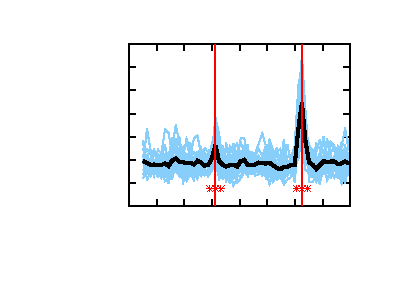
\includegraphics{./Figure_ITPC/itpc_anan}}%TL
    \put(3000,2300){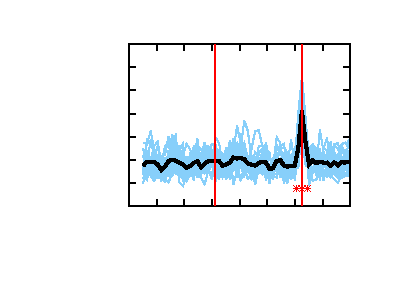
\includegraphics{./Figure_ITPC/itpc_avav}}%TR    
    \put(0,0){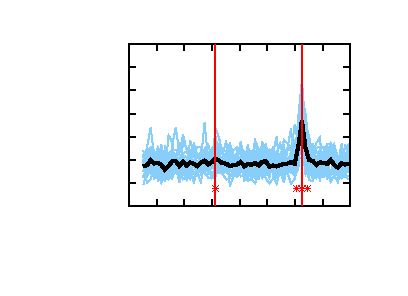
\includegraphics{./Figure_ITPC/itpc_phmi}}%BL
    \put(3000,0){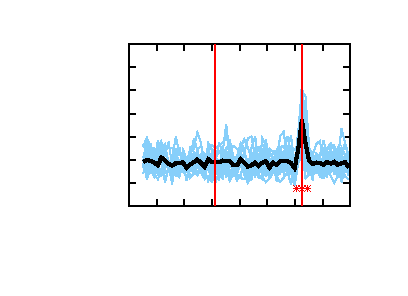
\includegraphics{./Figure_ITPC/itpc_rrrr}}%BR
    \gplfronttext
  \end{picture}%
\endgroup

\caption{EEG responses recorded in human participants for each of the
  four conditions. Statistically significant peaks in ITPC values were
  observed at the rate of syllable presentation (3.125 Hz) in each of
  the four conditions (AN, AV, MP, RR). A statistically significant
  peak in ITPC is observed at the rate of phrase presentation (1.5625
  Hz) in the AN and MP conditions. Red stars
  represent statistical significance $\star: p<0.05$, $\star\star: p<0.01$ and
  $\star\star\star: p<0.005$. Vertical red lines represent the
  frequency at which syllables and two-word sequences are presented.}
\label{fig:Fig2}
\end{figure}

In order to directly compare the ITPC values at the phrase rate across
the four conditions, the Kruskal-Wallis test was used. The effect of
condition was significant at the phrase frequency
($p=0.003$). Pairwise comparisons (one-sided pairwise Wilcoxon
signed-rank test, uncorrected) showed that the ITPC in the AN
condition at the phrase rate was significantly higher than in the AV
or MP condition (both $p=0.006$); the difference (two-sided pairwise
Wilcoxon signed-rank test) between the AN and MP condition was not
significant ($p=0.82$). Surprisingly the effect of condition on
syllable frequency was marginally significant ($p=0.051$) and the
pair-wise two-sided tests indicate that AV was different from RR
($p=0.0042$) and both AV ($p=0.041$) and AN ($p=0.0025$) were
different from MP. This might indicate that the participants listened
more attentively to the AN and AV stimuli.


Figure~\ref{fig:Fig3} shows individual particpants ITPCs for each
condition. Statistically significant peaks at the rate of syllable
presentation were observed in all participants in the AN and AV
conditions, 19/20 participants in the MP condition and 15/16 in the RR
condition.

When analysing the EEG responses of individual subjects at the rate of
phrase presentation, a statistically significant peak was observed in
14/20 participants in the AN condition, in 7/20 participants in the AV
condition, 9/20 in the MP and 3/16 in the RR conditions. Thus the
pattern observed in the grand averages can be seen in the majority of
individual participants.

\begin{figure}[tbhp]
%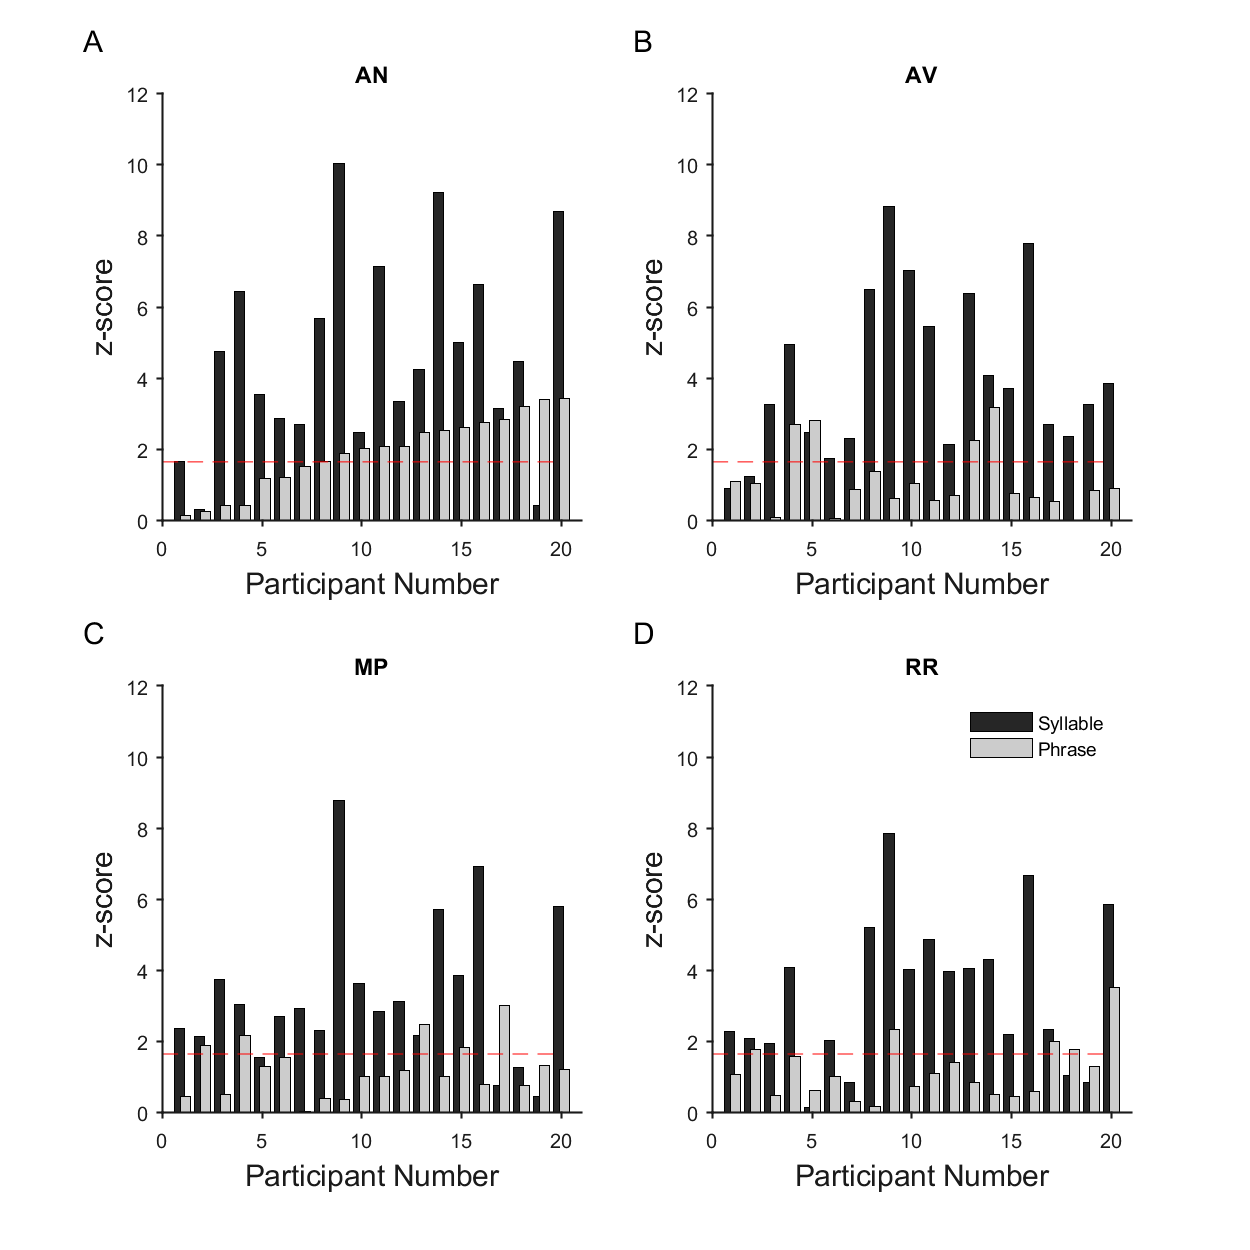
\includegraphics[width=\linewidth]{Exp2_individual_results_bar_graphs_thick.png}
% GNUPLOT: LaTeX picture with Postscript
\begingroup
  \makeatletter
  \providecommand\color[2][]{%
    \GenericError{(gnuplot) \space\space\space\@spaces}{%
      Package color not loaded in conjunction with
      terminal option `colourtext'%
    }{See the gnuplot documentation for explanation.%
    }{Either use 'blacktext' in gnuplot or load the package
      color.sty in LaTeX.}%
    \renewcommand\color[2][]{}%
  }%
  \providecommand\includegraphics[2][]{%
    \GenericError{(gnuplot) \space\space\space\@spaces}{%
      Package graphicx or graphics not loaded%
    }{See the gnuplot documentation for explanation.%
    }{The gnuplot epslatex terminal needs graphicx.sty or graphics.sty.}%
    \renewcommand\includegraphics[2][]{}%
  }%
  \providecommand\rotatebox[2]{#2}%
  \@ifundefined{ifGPcolor}{%
    \newif\ifGPcolor
    \GPcolorfalse
  }{}%
  \@ifundefined{ifGPblacktext}{%
    \newif\ifGPblacktext
    \GPblacktexttrue
  }{}%
  % define a \g@addto@macro without @ in the name:
  \let\gplgaddtomacro\g@addto@macro
  % define empty templates for all commands taking text:
  \gdef\gplbacktext{}%
  \gdef\gplfronttext{}%
  \makeatother
  \ifGPblacktext
    % no textcolor at all
    \def\colorrgb#1{}%
    \def\colorgray#1{}%
  \else
    % gray or color?
    \ifGPcolor
      \def\colorrgb#1{\color[rgb]{#1}}%
      \def\colorgray#1{\color[gray]{#1}}%
      \expandafter\def\csname LTw\endcsname{\color{white}}%
      \expandafter\def\csname LTb\endcsname{\color{black}}%
      \expandafter\def\csname LTa\endcsname{\color{black}}%
      \expandafter\def\csname LT0\endcsname{\color[rgb]{1,0,0}}%
      \expandafter\def\csname LT1\endcsname{\color[rgb]{0,1,0}}%
      \expandafter\def\csname LT2\endcsname{\color[rgb]{0,0,1}}%
      \expandafter\def\csname LT3\endcsname{\color[rgb]{1,0,1}}%
      \expandafter\def\csname LT4\endcsname{\color[rgb]{0,1,1}}%
      \expandafter\def\csname LT5\endcsname{\color[rgb]{1,1,0}}%
      \expandafter\def\csname LT6\endcsname{\color[rgb]{0,0,0}}%
      \expandafter\def\csname LT7\endcsname{\color[rgb]{1,0.3,0}}%
      \expandafter\def\csname LT8\endcsname{\color[rgb]{0.5,0.5,0.5}}%
    \else
      % gray
      \def\colorrgb#1{\color{black}}%
      \def\colorgray#1{\color[gray]{#1}}%
      \expandafter\def\csname LTw\endcsname{\color{white}}%
      \expandafter\def\csname LTb\endcsname{\color{black}}%
      \expandafter\def\csname LTa\endcsname{\color{black}}%
      \expandafter\def\csname LT0\endcsname{\color{black}}%
      \expandafter\def\csname LT1\endcsname{\color{black}}%
      \expandafter\def\csname LT2\endcsname{\color{black}}%
      \expandafter\def\csname LT3\endcsname{\color{black}}%
      \expandafter\def\csname LT4\endcsname{\color{black}}%
      \expandafter\def\csname LT5\endcsname{\color{black}}%
      \expandafter\def\csname LT6\endcsname{\color{black}}%
      \expandafter\def\csname LT7\endcsname{\color{black}}%
      \expandafter\def\csname LT8\endcsname{\color{black}}%
    \fi
  \fi
  \setlength{\unitlength}{0.0500bp}%
  \begin{picture}(6000.00,5000.00)%
    \gplgaddtomacro\gplbacktext{%
      \csname LTb\endcsname%


      \put(946,966){\makebox(0,0)[r]{\strut{} 0.1}}%
      \put(946,1363){\makebox(0,0)[r]{\strut{} 0.3}}%
      \put(946,1760){\makebox(0,0)[r]{\strut{} 0.5}}%
      \put(946,2157){\makebox(0,0)[r]{\strut{} 0.7}}%
      \put(1632,484){\makebox(0,0){\strut{}5}}%
      \put(2123,484){\makebox(0,0){\strut{}10}}%
      \put(2614,484){\makebox(0,0){\strut{}15}}%
      \put(3105,484){\makebox(0,0){\strut{}20}}%
      \put(376,1680){\rotatebox{-270}{\makebox(0,0){\strut{}ITPC}}}%      
      \put(2140,154){\makebox(0,0){\strut{}participant number}}%
      \put(2141,2400){\makebox(0,0){\strut{} \bf{MP}}}%             

      \put(3946,966){\makebox(0,0)[r]{\strut{} 0.1}}%
      \put(3946,1363){\makebox(0,0)[r]{\strut{} 0.3}}%
      \put(3946,1760){\makebox(0,0)[r]{\strut{} 0.5}}%
      \put(3946,2157){\makebox(0,0)[r]{\strut{} 0.7}}%
      \put(4632,484){\makebox(0,0){\strut{}5}}%
      \put(5123,484){\makebox(0,0){\strut{}10}}%
      \put(5614,484){\makebox(0,0){\strut{}15}}%
      \put(6105,484){\makebox(0,0){\strut{}20}}%      
%      \put(3176,1480){\rotatebox{-270}{\makebox(0,0){\strut{}ITPC}}}%
      \put(5140,154){\makebox(0,0){\strut{}participant number}}%
      \put(5141,2400){\makebox(0,0){\strut{} \bf{RR}}}%             

      \put(946,3266){\makebox(0,0)[r]{\strut{} 0.1}}%
      \put(946,3663){\makebox(0,0)[r]{\strut{} 0.3}}%
      \put(946,4060){\makebox(0,0)[r]{\strut{} 0.5}}%
      \put(946,4457){\makebox(0,0)[r]{\strut{} 0.7}}%
      \put(1632,2784){\makebox(0,0){\strut{}5}}%
      \put(2123,2784){\makebox(0,0){\strut{}10}}%
      \put(2614,2784){\makebox(0,0){\strut{}15}}%
      \put(3105,2784){\makebox(0,0){\strut{}20}}%
      \put(376,3980){\rotatebox{-270}{\makebox(0,0){\strut{}ITPC}}}%
            \put(2141,4700){\makebox(0,0){\strut{} \bf{AN}}}%      
 %     \put(2140,2154){\makebox(0,0){\strut{}frequency, Hz}}%

      \put(3946,3266){\makebox(0,0)[r]{\strut{} 0.1}}%
      \put(3946,3663){\makebox(0,0)[r]{\strut{} 0.3}}%
      \put(3946,4060){\makebox(0,0)[r]{\strut{} 0.5}}%
      \put(3946,4457){\makebox(0,0)[r]{\strut{} 0.7}}%
      \put(4632,2784){\makebox(0,0){\strut{}5}}%
      \put(5123,2784){\makebox(0,0){\strut{}10}}%
      \put(5614,2784){\makebox(0,0){\strut{}15}}%
      \put(6105,2784){\makebox(0,0){\strut{}20}}%
                  \put(5141,4700){\makebox(0,0){\strut{} \bf{AV}}}%             
 %     \put(3176,4480){\rotatebox{-270}{\makebox(0,0){\strut{}ITPC}}}%
 %     \put(5140,2154){\makebox(0,0){\strut{}frequency, Hz}}%
}%
    \gplgaddtomacro\gplfronttext{%
    }%
    \gplbacktext
    \put(0,2300){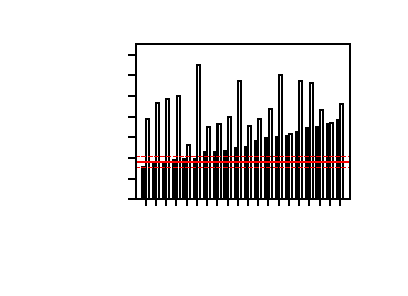
\includegraphics{./Figure_Individuals/anan}}%TL
    \put(3000,2300){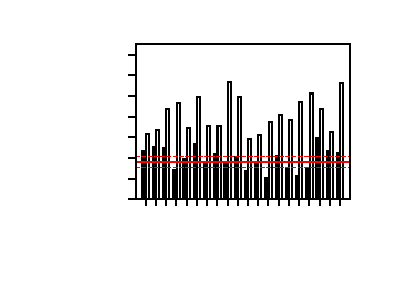
\includegraphics{./Figure_Individuals/avav}}%TR    
    \put(0,0){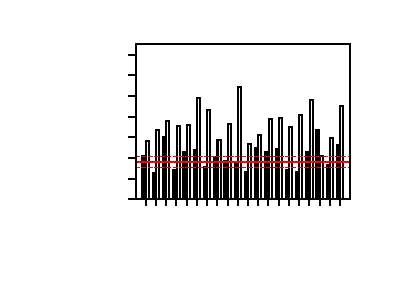
\includegraphics{./Figure_Individuals/phmi}}%BL
    \put(3000,0){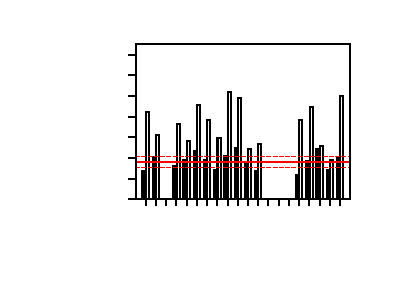
\includegraphics{./Figure_Individuals/rrrr}}%BR
    \gplfronttext
  \end{picture}%
\endgroup



\caption{ITPC responses from individual participants at the phrase
  rate (3.125 Hz; filled bars) and the syllable rate (1.5625 Hz;
  unfilled bars) in each of the four conditions (AN, AV, MP, RR). For
  the AN, AV and MP conditions, values of the ITPC at each frequency
  of interest are displayed for each of the 20 participants, for RR,
  for the 16 participants. Participants one to 20 are ordered in
  accordance to their ITPC at the phrase frequency in the AN
  condition, in increasing order from left to right. Red horizontal
  lines indicate the mean ITPC value for random phases along with the
  corresponding significance thresholds (p < 0.05) and so any ITPC
  that is above the upper red line is significantly higher than chance
  level.}
\label{fig:Fig3}
\end{figure}


\section*{Discussion}


The current study investigated whether, and to what extent, syntactic
structure is automatically utilised by the brain during language
comprehension, over and above information about grammatical
category. It was found that repetitive presentation of grammatically
well-formed, two-word adjective-noun phrases yields a prominent peak
in ITPC at the rate of phrase presentation, but that repetitive
presentation of two-word adjective-verb sequences that cannot be
combined into a phrase did not produce a peak. The amplitude of the AN
peak, as well as the syllable peak in response to single words, is
consistent with previous findings \citet{DingEtAl2017}. This provides
support for a syntactic operation that enables combining of words into
higher-level syntactic units and suggests that the processing of
linguistic input involves levels of abstraction beyond word-level
grammatical-category information. This supports classical syntax-based
approaches to language
\citet{BerwickEtAl2013,EveraertEtAl2015,Chomsky1995}. It is also
generally compatible with the proposal that higher-level chunking of
smaller language units occurs during language processing
\citet{ChristiansenChater2016}, although the nature of what the chunks
are remains unclear. Indeed, in our analysis we have assumed that the
grammatical categories we employed in designing our stimuli are
relevant for language processing in the brain. There are other
grammatical accounts that could be used to construct putative phrase
conditions. Nonetheless, using a Chomskyan account of phrase structure
has given us two conditions, AN and AV, which produced significantly
different responses.

The distributional semantics model predicts a similar peak in ITPC at
the rate of phrase presentation during both the AN and AV
conditions. However, despite similarity in distributional vector space
for the AN and AV conditions, the ITPC peak at the rate of phrase
presentation was absent in the AV condition in the experimental
recording. This suggests that the brain's response is not merely a
function of grammatical category; rather, it also reflects
higher-level syntactic constituency.

The ITPC peak at the rate of phrase presentation was found in response
to the MP condition was significantly smaller than the peak found in
response to the AN condition, even though the MP condition contained
repeated presentation of grammatically well-formed phrases. To the
extent that each phrase involves combining two words into a single
syntactic unit, there is a clear regularity in the MP condition at the
syntactic level. This reduction might indicate that the response is
not sufficiently abstract to reflect repetition of syntactic
constituents independent of their lexical properties; for example, the
phrases differ in the location of their head; determiner-noun phrases
have the head after the modifier (\texttt{that word}) while
verb-adverb phrases have their head before (\texttt{send
  less}). According to this interpretation, the phrase-level response
found in the AN condition cannot be interpreted in its entirety as a
reflection of the Merge operation \citet{Chomsky1995} in its most
general form: in both the AN and MP conditions words are pairwise
merged into a phrase, but the ITPC peak is larger in the former case.

Another explanation for the reduction in phrase peak in the response
to the MP condition is that streams for this condition are more
difficult to follow and consequently less well attended to. To
investigate this we performed a behavioural study in which subjects
listened to a stimulus modelled on our EEG stimulus with streams for
the AN, MP and RR condition. After the last stream they were asked to
indicate whether they thought the last stream was composed of two-word
phrases or random words. The order of the streams was randomized, thus
each subject was only asked this question about one condition with a
given subject had an equal chance of being asked about each condition:
the AN, MP or RR stream; in fact there were 33 subjects asked about an
AN stream, 27 about an MP stream and 28 about an RR stream.

For AN $32/33\approx 0.97$ thought the stream was made of two-word
phrases, for MP this was $24/27\approx 0.89$ and for RR it was
$22/28\approx 0.79$. Thus, almost all subjects asked about an AN
stream correctly identified that is was composed of phrases, but a
substantial majority of subjects asked about an RR stream incorrectly
believed it was in fact composed of phrases; MP lies between the
two. A Fisher Exact test shows that AN subjects were significantly
($p=0.031$) more likely to believe the stream was composed of phrases
than RR subjects; the other two comparisons are not significant
(AN$>$MP $p=0.234$ and MP$>$RR $p=0.253$). This behavioural experiment
demonstrates the difficulty in parsing the stimulus as it is being
listened to and does indicate that the MP streams are harder to
distinguish from RR than the AN streams. See the Supplementary
Information for a description of the design of this experiment.

A model of language comprehension is likely to exploit linear and
hierarchical factors and describe how the brain uses different types
of evidence: lexical, syntactic and semantic, in deducing
meaning. While these different elements had seemed difficult to
reconcile, recent neural network models with a linear temporal
structure are able to discover and encode hierarchical structure, see
\citet{LakretzEtAl2019,Baroni2019} for example. These models are
consistent with the results outlined in the current study. Here we
present evidence that words are combined by the brain into phrases and
that syntactic information is important for the brain's response to
language; this indicates that hierarchical structure is deduced and
classified, at least in part, based on syntactic information.

One issue with frequency tagging experiments, like the one presented
here, is that neural mechanisms responsible for generating the ITPC in
the frequency tagging paradigm are still not clear. It may be that
cortical entrainment to the rate at which features of interest are
presented causes the peaks in ITPC \cite{Meyer2018}, or instead it is
possible that the frequency tag is driven by regularities in ERPs in
response to individual words or their combination. It is also possible
that there is a variable `error' signal associated with the
irregularity of the MP condition and the ill-formed AV phrases and
this is disrupting the response at 1.5625 Hz, the phrase
frequency. Indeed, without a model relating neural dynamics to the
ITPC we cannot be certain that the relative sizes of different
responses are indicative of different manipulations of the incoming
signal; this is a limitation of frequency-tagged experiments such as
the one presented here.

In \citet{PulvermullerEtAl2002} it is argued that specific networks of
neurons may be sensitive to sequences of words from discrete
grammatical categories. In this way, local networks of neurons could
learn to become sensitive to activation by a sequence of elements from
different groups, for example an adjective followed by a noun, as in
the AN condition presented in this study. This could explain why we
see a larger ITPC at the phrase rate following repetitive presentation
of phrases of the same type (AN). In other words adjective-noun
sequences would repetitively and consistently activate the same
sequence-detecting network of neurons responsible for processing
adjective-noun sequences, whereas presentations of a mixture of
different types of phrases would activate a different network of
sequence-detecting neurons and thus generate an inconsistent EEG
response and a smaller peak in ITPC at the phrase rate. On the other
hand there would be no sequence-detector network for ungrammatical
combinations, such as adjective-verb, and these therefore fail to
elicit a phrase-level response.

In conclusion, the experiments described in the current study
demonstrate that neural entrainment cannot be readily explained at the
lexical level; rather, it additionally calls for higher-level
syntactic representations. Yet, in our paradigm, frequency tagging of
higher-level syntactic units emerged most strongly in the presence of
grammatical category repetition, leaving open the question of how
abstract syntactic representations are.

\section*{Methods}
\subsection*{Participants}

Twenty right-handed, native English speakers (12 female, mean age 25
years, range 22 - 42 years) participated in this study. Participants
were screened for dyslexia and hearing impairments. All participants
gave written, informed consent prior to undertaking the study and were
reimbursed for their time at a rate of £10/hour. Ethical approval for
our experimental procedures were obtained from the University of
Bristol Faculty of Science ethics board. All methods were performed in
accordance with the relevant guidelines and regulations.

\subsection*{Stimuli}

The experimental procedures were similar to those used in a recent EEG
study \cite{DingEtAl2017}. Listeners were played streams of
monosyllabic words in English. The words were synthesised individually
using the \texttt{MacinTalk Synthesizer} (male voice \texttt{Alex}, in
\texttt{Mac OS X 10.7.5}). All of the synthesised words (226 - 365 ms)
were adjusted to 320 ms duration and normalised in intensity using the
freely available \texttt{Praat} software \citet{Praat}.

Monosyllabic words were selected from different grammatical categories,
namely adjectives, nouns, verbs, pronouns, adverbs, determiners and
prepositions. Words were only selected if they could be unambigouously
categorised into a distinct grammatical category, so, for example
words such as \texttt{drink}, \texttt{ride} or \texttt{walk} were
avoided because they are ambiguous between verbs and nouns. All nouns
were singular and all verbs were in the present tense.

The four experimental conditions were AN, AV, MP and RR:
\begin{enumerate}
\item Repetition of `adjective-noun' sequences (AN). 
\begin{center}
\text{\myuline{cold food}\tts\myuline{loud room}\tts\myuline{tall girl}\tts\myuline{bad cat}\tts\myuline{huge car}}
\end{center}
An adjective and a noun were repeated every other word. This condition
contained grammatically correct two-word phrases, (underlined, with the
grammatical category repeated every second word.

\item Repetition of `adjective-verb' sequences (AV).
\begin{center}
\text{\texttt{rough give ill tell thin chew hot hang green fetch}}
\end{center}
An adjective and a verb were repeated every other word. The word
sequence in this condition preserved the repetition of grammatical
category but did not contain grammatically well-formed phrases.

\item Repetition of grammatically well-formed phrases (underlined) without repetition of grammatical category information (MP).
\begin{center}
\text{\myuline{that word}\tts\myuline{send less}\tts\myuline{not loud}\tts\myuline{huge bird}\tts\myuline{fish cry}}
\end{center}
Grammatically well-formed, two-word phrases were composed from a pool
of adjectives, nouns, verbs, pronouns, adverbs, determiners and
prepositions. Phrases could take one of the following forms:
`verb-noun', `verb-adjective', `adverb-adjective', `determiner-noun',
`preposition-noun', `verb-adverb' and these were presented in a
pseudo-randomised order to avoid repetition of grammatical category in
adjacent phrases and to prevent grammatical phrases occurring across
phrase boundaries: thus, for example, \myuline{not loud} \myuline{fish
  cry} would be excluded since \myuline{loud fish} is a noun phrase.

\item Pseudo-random word sequence chosen so that no phrases can be formed regularly between adjacent words.
\begin{center}
\label{eq:RR}
\text{\texttt{with chew small the his out tall old down tell}}
\end{center}
In this condition, words from the pool of adjectives, verbs, prepositions and determiners were randomly selected. Nouns were not included because they combine into grammatically correct phrases with words from many other grammatical categories.
\end{enumerate}

A complete list of all stimuli used in the current study can be found
in the Supplementary Information. Critically, in the AN and AV
conditions, words were ordered such that there is not difference in
similarity between the word2vec representation of consecutive
words. Taking AN as an example, all the cosine similarities between
the vectors representing adjective and nouns were calculated and only
those pairs with values between 0.75 and one were retained; these values
were hand-tuned to give a sufficient number of pairs while excluded as
far as possible dissimilar pairs. To form a stream an initial pair was
picked for this set, giving the first adjective-noun pair in the
stream, $A_1$ and $N_1$. The adjective, $A_2\not=A_1$, whose similarity
to $N_1$ is closest to the similarity of $A_1$ and $N_1$ is then
picked. Next the noun $N_2$ is picked so its similarity to $A_2$ the
closest to the similarity of $N_1$ and $A_2$. With the constraint that
no pair appears twice, this is repeated until all 52 words are
chosen. The same method was used to generate streams for the AV
condition.

%Which "word representations? Was this done for all A and N pairings
%only (ie A-A pairings and N-N pairings were not taken into account,
%correct?) It's worth spelling things like this out more explicitly

\subsection*{Experimental Procedures}

Each stream contained a sequence of 52 monosyllabic words played back
to back in a continuous stream. Streams were therefore 16.64 seconds
long. In total, participants listened to 150 streams, with 25 streams
for each of the four conditions AN, AV, MP and RR, along with two
filler conditions. An error in the marker file meant that one block
was not usable, so 24 streams were included in the analysis. Blocks
were made up of six streams and contained one stream from each condition
plus the two filler streams. Within each block, streams were presented
to the participants one after the other. After each stream,
participants were asked whether they had heard any four word phrases,
the instructions give three examples: \myuline{ask him this thing},
\myuline{from my old car} or \myuline{sit in that tree}. This acted as
the attention trap with the four-word phrases occurred in ten percent
of streams. These streams were not excluded from the analysis. Following
the button press, the next stream was played after a delay of 250
ms. At the end of each block participants were given a 10s break, with
a longer 2 minute break at the halfway point. The streams within each
block were presented in a random order that was counterbalanced across
participants but the composition of blocks and their order was the
same across participants.

\subsection*{EEG Recording}
 
EEG signals were sampled at 1000 Hz from 32 Ag/AgCl electrodes fitted
on a standard electrode layout elasticised cap using a BrainAmp DC
amplifier (Brain Products GmbH). The EEG was recorded in DC mode ,
using a low-pass filter of 1000 Hz (fifth-order Butterworth filter
with 30 dB/octave)-. FCz was used as a reference channel. The
impedance of the electrodes was kept below 5 kOhms. Recordings were
analysed offline using \texttt{Matlab} (Mathworks Inc.) and the
\texttt{Fieldtrip} toolbox \cite{FieldTrip}. As the recordings were
performed using a 32-channel system (rather than a 128-channel system
as, for example, \citet{DingEtAl2017}) we did not do dimensional
reduction on our EEG signals using PCA. Eyeblink artifacts were
removed by applying ICA to the filtered signal. An independent
component was removed if in its topography the mean power over the
most frontal four channels (Fp1, Fp2, F7 and F8) was two times greater
than the mean power over all other channels, as in
\citet{DingEtAl2017}. As our signals of interest are in the
low-frequency region, at 1.5625 Hz (phrases), and 3.125 Hz
(syllables), the EEG signals were filtered offline using a 25 Hz
low-pass filter (sixth-order Butterworth IIR). Data were re-referenced
offline to a common average reference. For each condition, individual
streams (16.64s long) were epoched. Upon sound onset there is a
transient EEG response and so the first four syllables (1.28 seconds)
in each epoch were removed from the analysis. This meant that the
overall length of the analysed part of each stream was 15.36 seconds
(corresponding to 48 syllables x 0.32 s).

\subsection*{Data analysis}

After preprocessing, the EEG signal was converted into the frequency
domain using the discrete Fourier transform with a frequency
resolution of 0.0651 (1/15.36) Hz. The intertrial phase coherence
(ITPC), what is also known as the square mean resultant, is
\begin{equation}
\label{eq:itpc}
R(f;\phi)=\frac{\left|\sum_k e^{i\theta_{k\phi}}\right|}{K}
\end{equation}
where $\theta^c$ is the phase angle of each complex-valued Fourier
coefficient at frequency $f$ and $k$ is a trial index, with $\phi$
representing the other parameters such as the channel.

In most examples, the ITPC is calculated for each of the four
different conditions for each participant and each channel; in this
case $k$ represents the different word streams corresponding to a
given condition. In this case the ITPC is $R(f;pce)$ where $p$ labels
participants, $c$ conditions and $e$ electrodes. This is averaged across
electrodes to give $R(f;pc)$ and, for example, the ITPC for different
conditions is compared by examining the 20 pairs of values
corresponding to the twenty partipants. For the `per-item' analysis
the ITPC is calculated for each condition for each stream and each
channel so that $k$ corresponds to the different participants. After
also averaging across electrodes, this gives $R(f;sc)$ where $s$ is
the index which labels t.

\subsection*{Significance Testing}

To determine whether a peak at one of the two target frequencies was
significantly different from chance the ITPC was compared to the ITPC
for random data. For the data an ITPC was calculated for each
electrode using 24 phases computed for the 24 streams in each
condition for the stimulus; this is then averaged over the 32
electrodes. To produce a simulated ITPC this calculation was mimicked
for random phases. Thus, 24 phases were picked at random and used to
calculate a ITPC for one `electrode', this was repeated 32 times and
the 32 values were averaged to give a simulated ITPC value which can
be compared to the ITPC values calculated using the experimental
data. To produce the confidence intervals for Fig.~\ref{fig:Fig3}
5,000 of these simulated ITPC values were generated in this way, these
were ordered and, for example, the 95\% confidence interval
corresponds to the 250th and 4750th entries in this list. To determine
whether an ITPC peak was significantly different from chance a
Mann-Whitney U-test was performed using these 5,000 values and the
actual participant data.

\subsection*{Simulating Word Vector ITPCs}

The word2vec repsententions for the words used in the stimuli were
downloaded from
(\url{https://fasttext.cc/docs/en/pretrained-vectors.html}). These
were calculated using a distributional semantics model that was
trained on a large English corpus \citet{Bojanowski2017}. Following
\cite{FrankYang2018} the simulated EEG was calculated from these
vectors: the vectors are 300-dimensional so they give 300 channels.
Time is discretized into 1ms quanta and a period of 320ms is allocated
to each word. For a given stream let $v_e(t)$ denote the value of the
voltage at time $t$. If $\textbf{w}^1$ is the word2vec representation
of the first word in the stream then for $t\in [1,320]$
\begin{equation}
  v_e(t)=\left\{\begin{array}{ll}\eta\xi(t)&t<\tau\\ w^1_e+\eta\xi(t)\end{array}\right.
\end{equation}
where $\tau$ is a delay chosen uniformly in the interval [20,60],
$\xi(t)$ is unit-variance zero-mean pink-noise and $\eta=0.5$. This is
repeated for each word in the stream, with independent
$\tau$. Individual participants correspond to a different random
selection of 32 `electrodes' from the 300 components and to different
instances of the $1/f$-noise: this is done to give the graphs some
similarity to the graphs for the real data, but is not intended to
model participant-to-participant variability.

The AN, AV and MP conditions use the identical stimuli as used in the
experiment. However, the random condition differs from the RR
condition in that the words are shuffled. In the RR condition adjacent
words are chosen so as to not repeat grammatical category, the ITPC on
these data is sensitive enough to detect this deviation from true
randomness. With its different types of artificial noise, the
simulated EEG is a complicated measure of the regularity of the
stimuli. A much simpler measure is given by the Fourier coefficent
\begin{equation}
  \phi= \sum_e\left|\sum_i (-1)^iw_e^i\right|
\end{equation}
where $w_e^i$ is the $e$ component of the $i$th word in a
stream. Averaging $\phi$ over streams and normalizing to the random
condition gives values of 1.87, 2.41, 1.41, 1.13 for AN, AV, MP and RR
respectively.


\section*{Code and data availability}
The data collected in this study is available at
\texttt{doi:10.5281/zenodo.4019709}; the \texttt{Presentation 20.0}
(Neurobehavioural Systems Inc.) script used to run the experiment, the
stimuli and the code used for data analysis and for producing the
simulated EEG is available at \texttt{doi:10.5281/zenodo.4275804}. In
addition to the \texttt{Matlab} code used to epoch the EEG data,
perform blink-removal and calculate the Fourier transform, analysis
and simulations were performed using \texttt{Julia 1.1.1}. All data
from the behaviour experiment and the scripts in \texttt{jsPsych
  5.0.1} used to run the experiment are available online at
\texttt{doi:10.5281/zenodo.4275815}.

\section*{Competing Interests}
The authors declare that no competing interests exist.

\bibliography{references}{}

\section*{Author Contributions}
AB, NK and CJH contributed to the conception and design of the work;
AB carried out the experiments, AB and CJH performed the analysis and
prepared the figures. AB wrote the initial draft of the main
manuscript text, CJH and NK made a significant contribution during
manuscript revisions.

\end{document}

